\section{Requirements and Message Protocol}
\label{sec:protocol}

\subsection{Lines of at most 32 bytes, each answered exactly once}
The link is USART1 on PA9 (TX) and PA10 (RX) through the ST-Link virtual COM port, 115200 baud, 8N1,
no flow control. A \emph{frame} is \code{body[*HH]} followed by LF (Table~\ref{tab:framing}). The body is
printable ASCII; \code{HH} is the XOR of all body bytes as two uppercase hex digits. Replies always
carry it; requests may omit it so a person can type into a terminal, but a wrong one is rejected.
Every frame, whether complete, oversize or timed out, gets exactly one reply, and the server
never speaks unprompted.

\begin{table}[t]
\centering
\caption{Framing rules and the server's response to each violation.}
\label{tab:framing}
\footnotesize
\begin{tabular}{@{}L{2.6cm}L{5.4cm}@{}}
\toprule
Rule & Server behaviour \\
\midrule
Terminator & LF ends a frame; one CR before it is dropped \\
Maximum length & 32 bytes before the LF; the 33rd byte gives \code{NACK:TOOLONG} at once, the rest is skipped silently to the next LF \\
Incomplete frame & 500 ms without a byte: \code{NACK:TIMEOUT} (silent while skipping) \\
Invalid character & Empty frame or byte outside 0x20--0x7E: \code{NACK:BADCMD} \\
Checksum & Malformed or wrong \code{*HH}: \code{NACK:BADSUM} \\
\bottomrule
\end{tabular}
\end{table}

A frame is checked in a fixed order and the first failure wins: length, printable, checksum, then command syntax.
Only a frame that passes all four reaches the game state machine, so no framing error can touch game state.

\subsection{The board is nine characters}
The board is nine characters, cells 0--8 left to right, top to bottom: \code{.} empty, \code{X}, \code{O}.
\code{XO.XO....} has X at cells 0 and 3 and O at 1 and 4. X always moves first, and the side to move is X when
the counts are equal, otherwise O, so a client can derive it from the board alone.

\subsection{Seven commands, each defined in every state}
Table~\ref{tab:commands} lists the commands. The state table is total: all 18 command/state pairs of the six core commands have a defined
reply (\code{NEW:AI} follows the \code{NEW} row), and a valid command in the wrong state gets \code{NACK:NOGAME} when it needs a running game and
\code{NACK:STATE} otherwise. A game started or reset with the board's button sends nothing; the client finds out
on its next request (\code{MOVE} gives \code{NACK:NOGAME}) and returns to its start screen.

\begin{table}[t]
\centering
\caption{Command set. $^\dagger$ marks a departure from the brief.}
\label{tab:commands}
\scriptsize
\begin{tabular}{@{}L{2.25cm}L{1.95cm}L{3.8cm}@{}}
\toprule
Request & Accepted in & Success response \\
\midrule
\code{CONNECT} & IDLE & \code{OK} \\
\code{NEW} & IDLE, GAME\_OVER & \code{OK:BOARD:.........} \\
\code{NEW:AI}$^\dagger$ & IDLE, GAME\_OVER & \code{OK:BOARD:.........}; server plays O \\
\code{MOVE:<i>[:<m>]}$^\dagger$ & IN\_PROGRESS & \code{OK:BOARD:<9>}, or \code{WIN:<m>:BOARD:<9>}$^\dagger$, or \code{DRAW:BOARD:<9>}$^\dagger$ \\
\code{STATE} & IN\_PROGRESS, GAME\_OVER & \code{BOARD:<9>} \\
\code{RESIGN} & IN\_PROGRESS & \code{OK:GAMEOVER} \\
\code{DISCONNECT} & IDLE$^\dagger$, GAME\_OVER & \code{OK} \\
\bottomrule
\end{tabular}
\end{table}

\subsection{Nine NACK codes, checked in a fixed order}
Table~\ref{tab:errors} lists every error. Every NACK leaves board, turn and state unchanged. A \code{MOVE} that fails several
checks reports the first in this order: state, range, turn, occupancy. For example \code{MOVE:9:O} on X's turn is \code{NACK:RANGE}, so each request has one correct reply.

\begin{table}[t]
\centering
\caption{Every error response and when the server sends it.}
\label{tab:errors}
\footnotesize
\begin{tabular}{@{}L{2.35cm}L{5.65cm}@{}}
\toprule
Response & Sent when \\
\midrule
\code{NACK:TOOLONG}$^\dagger$ & Frame longer than 32 bytes \\
\code{NACK:TIMEOUT}$^\dagger$ & Partial frame, 500 ms without a byte \\
\code{NACK:BADSUM}$^\dagger$ & \code{*HH} malformed or wrong \\
\code{NACK:BADCMD} & Empty, non-printable, unknown command or bad argument (e.g.\ \code{MOVE:4X}) \\
\code{NACK:NOGAME} & Command needs a running game and none exists \\
\code{NACK:STATE}$^\dagger$ & Valid command, wrong state (e.g.\ \code{NEW} mid-game) \\
\code{NACK:RANGE} & Index outside 0--8 (\code{9}, \code{-1}) \\
\code{NACK:NOTURN} & Claimed mark is not the side to move \\
\code{NACK:OCCUPIED} & Target cell not empty \\
\bottomrule
\end{tabular}
\end{table}

\subsection{Six departures and one extension, each justified}
\begin{enumerate}\setlength\itemsep{0pt}
\item \emph{Terminal replies carry the board} (\code{WIN:X:BOARD:...}). The client redraws from one reply instead of paying a \code{STATE} round trip.
\item \emph{Optional \code{:<m>} on \code{MOVE}.} With one client an out-of-turn move cannot otherwise be sent, so \code{NACK:NOTURN} would be untestable. The GUI always sends the mark, so a stale client is detected.
\item \emph{Extra codes} \code{TOOLONG}, \code{TIMEOUT}, \code{BADSUM}, \code{STATE}, so framing and integrity failures are distinguishable from bad commands.
\item \emph{Checksum optional on requests}, mandatory on replies, to keep terminal testing possible.
\item \emph{\code{DISCONNECT} accepted in IDLE}, so a client that connected but never started can leave cleanly.
\item \emph{\code{STATE} in IDLE is \code{NACK:NOGAME}}, and \emph{\code{NEW} in progress is \code{NACK:STATE}} (resign first); the button is a local reset with no message.
\item \emph{Extension \code{NEW:AI}} starts a game in which the human is X and the server answers each accepted move with its own O move before replying, so the reply shows both moves and there is still one reply per frame. Plain \code{NEW} is unchanged, so clients that ignore the extension are unaffected.
\end{enumerate}

Figure~\ref{fig:sequence} shows both halves of the protocol. In (a) a game runs from \code{CONNECT} to an X win; the
move after the win is refused with \code{NACK:NOGAME}. In (b) the server refuses an occupied cell, an out-of-range index and
a corrupted request, and a following \code{STATE} shows the board unchanged.

\begin{figure*}[t]
\centering
% Two-panel sequence diagram. Solid = request (PC to STM32), dashed = reply.
\newcommand{\seqpair}[3]{% y, request, reply
  \draw[->,>=stealth] (0,#1) -- node[above=1.5pt,font=\fontsize{7}{8}\selectfont\ttfamily,inner sep=1pt]{#2} (3.7,#1);
  \draw[<-,>=stealth,dashed] (0,#1-0.5) -- node[above=1.5pt,font=\fontsize{7}{8}\selectfont\ttfamily,inner sep=1pt]{#3} (3.7,#1-0.5);}
\begin{minipage}[t]{0.49\linewidth}\centering
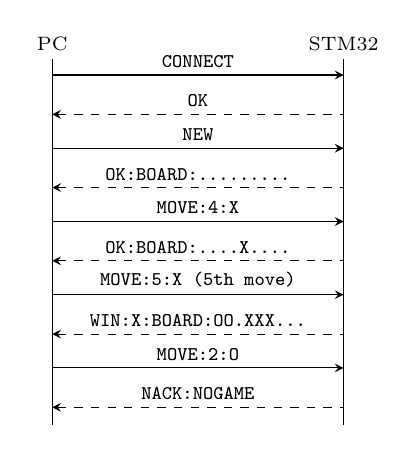
\begin{tikzpicture}[x=1cm,y=1cm]
 \node[font=\scriptsize] at (0,0.35) {PC};\node[font=\scriptsize] at (3.7,0.35) {STM32};
 \draw (0,0.15) -- (0,-4.5);\draw (3.7,0.15) -- (3.7,-4.5);
 \seqpair{-0.05}{CONNECT}{OK}
 \seqpair{-0.98}{NEW}{OK:BOARD:.........}
 \seqpair{-1.91}{MOVE:4:X}{OK:BOARD:....X....}
 \seqpair{-2.84}{MOVE:5:X (5th move)}{WIN:X:BOARD:OO.XXX...}
 \seqpair{-3.77}{MOVE:2:O}{NACK:NOGAME}
\end{tikzpicture}\\[2pt]{\footnotesize (a) X wins}
\end{minipage}\hfill
\begin{minipage}[t]{0.49\linewidth}\centering
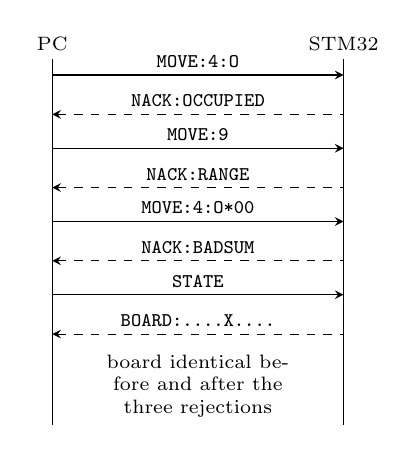
\begin{tikzpicture}[x=1cm,y=1cm]
 \node[font=\scriptsize] at (0,0.35) {PC};\node[font=\scriptsize] at (3.7,0.35) {STM32};
 \draw (0,0.15) -- (0,-4.5);\draw (3.7,0.15) -- (3.7,-4.5);
 \seqpair{-0.05}{MOVE:4:O}{NACK:OCCUPIED}
 \seqpair{-0.98}{MOVE:9}{NACK:RANGE}
 \seqpair{-1.91}{MOVE:4:O*00}{NACK:BADSUM}
 \seqpair{-2.84}{STATE}{BOARD:....X....}
 \node[font=\scriptsize,text width=3cm,align=center] at (1.85,-4.0) {board identical before and after the three rejections};
\end{tikzpicture}\\[2pt]{\footnotesize (b) rejections (board \code{....X....})}
\end{minipage}

\caption{Sequence diagrams (checksums omitted; solid = request, dashed = reply). (a)~A scripted X win. (b)~Three rejections leave the board unchanged.}
\label{fig:sequence}
\end{figure*}
